\paragraph{Peak alignment}
%The repeatability of the pSTAT MFI was assessed.  
Another approach to the normalisation as implemented in the \Rpackage{flowStats}, is to align the modes
of the distributions across days in the ungated sample.
The method assumes that the two peaks in the pSTAT5 distribution,
representing stimulated and unstimulated cells,
should exist in all ungated samples, while their locations and their proportions may vary across doses and days.
%Given that the location of the peaks of pSTAT5 in the ungated sample remains fairly stable across doses but that the heights vary,
%this advocates a normalisation method which relies on peak alignment.
%If we expect that the core cell populations should exist in all samples but that their locations and their proportions may vary across days and dose,
%a normalisation approach is to align the location of the population across doses per day.
%Hence we wish to align the location of the peaks across days while allowing for the relative proportion of the populations to vary.  
%The idea is to identify the groups based on a single marker by clustering algorithm and then selecting the peaks to be the group medians.
%In this approach the number of groups K needs to be known a priori and is assumed to be the same across samples.
%This is the method used by \Rpackage{flowBeads} which identifies groups with the k-medoids algorithm for the purpose of bead normalisation.
%In Chapter 3, I used k-means to identify the peaks, but I found on this data k-means and k-medoids performed poorly since the cluster variances are very different.  
Unfortunately in flow cytometry, the peaks are not always clearly identifiable due to noise associated with staining.
This is particularly noteable in ungated data where debris obfuscate the pSTAT5 signal and can introduce artefactual peaks, leading to peak misidentification.
Furthermore, the transform can also introduce spurious peaks close to zero.
In particular, the second peak corresponding to the stimulated cells is much broader and smaller since the majority of cells in the sample are not stimulated.
However I found that upon gating on lymphocytes and CD4\positive lymphocytes, these spurious peaks disappear and both peaks were correctly identified 
%A mixture model algorithm would be better suited since it allows for different variances in the clustering.
%but because of the skewness of the data, the peaks did not correspond to the cluster medians.
To identify the peaks, I used a sliding window approach on the density function.
The sliding window approach records the point with the highest density estimate in the current window,
so that within a window of twice the span, the point of highest density is selected as a peak.
At the end, a list of highest density points is returned of which the top two are selected.
I found in practice this method worked well with a window span of $40$ across all samples considered.
%This approach is useful for estimating K but the window size may need to be tuned per sample.  
%depending on the value of the width parameter selected for the logicle transform.
%(\Cref{appendix:transformation,appendix:normalisation}).
(\Cref{figure:pstat5-peak-normalisation}).
\begin{figure}[h]
    \centering
    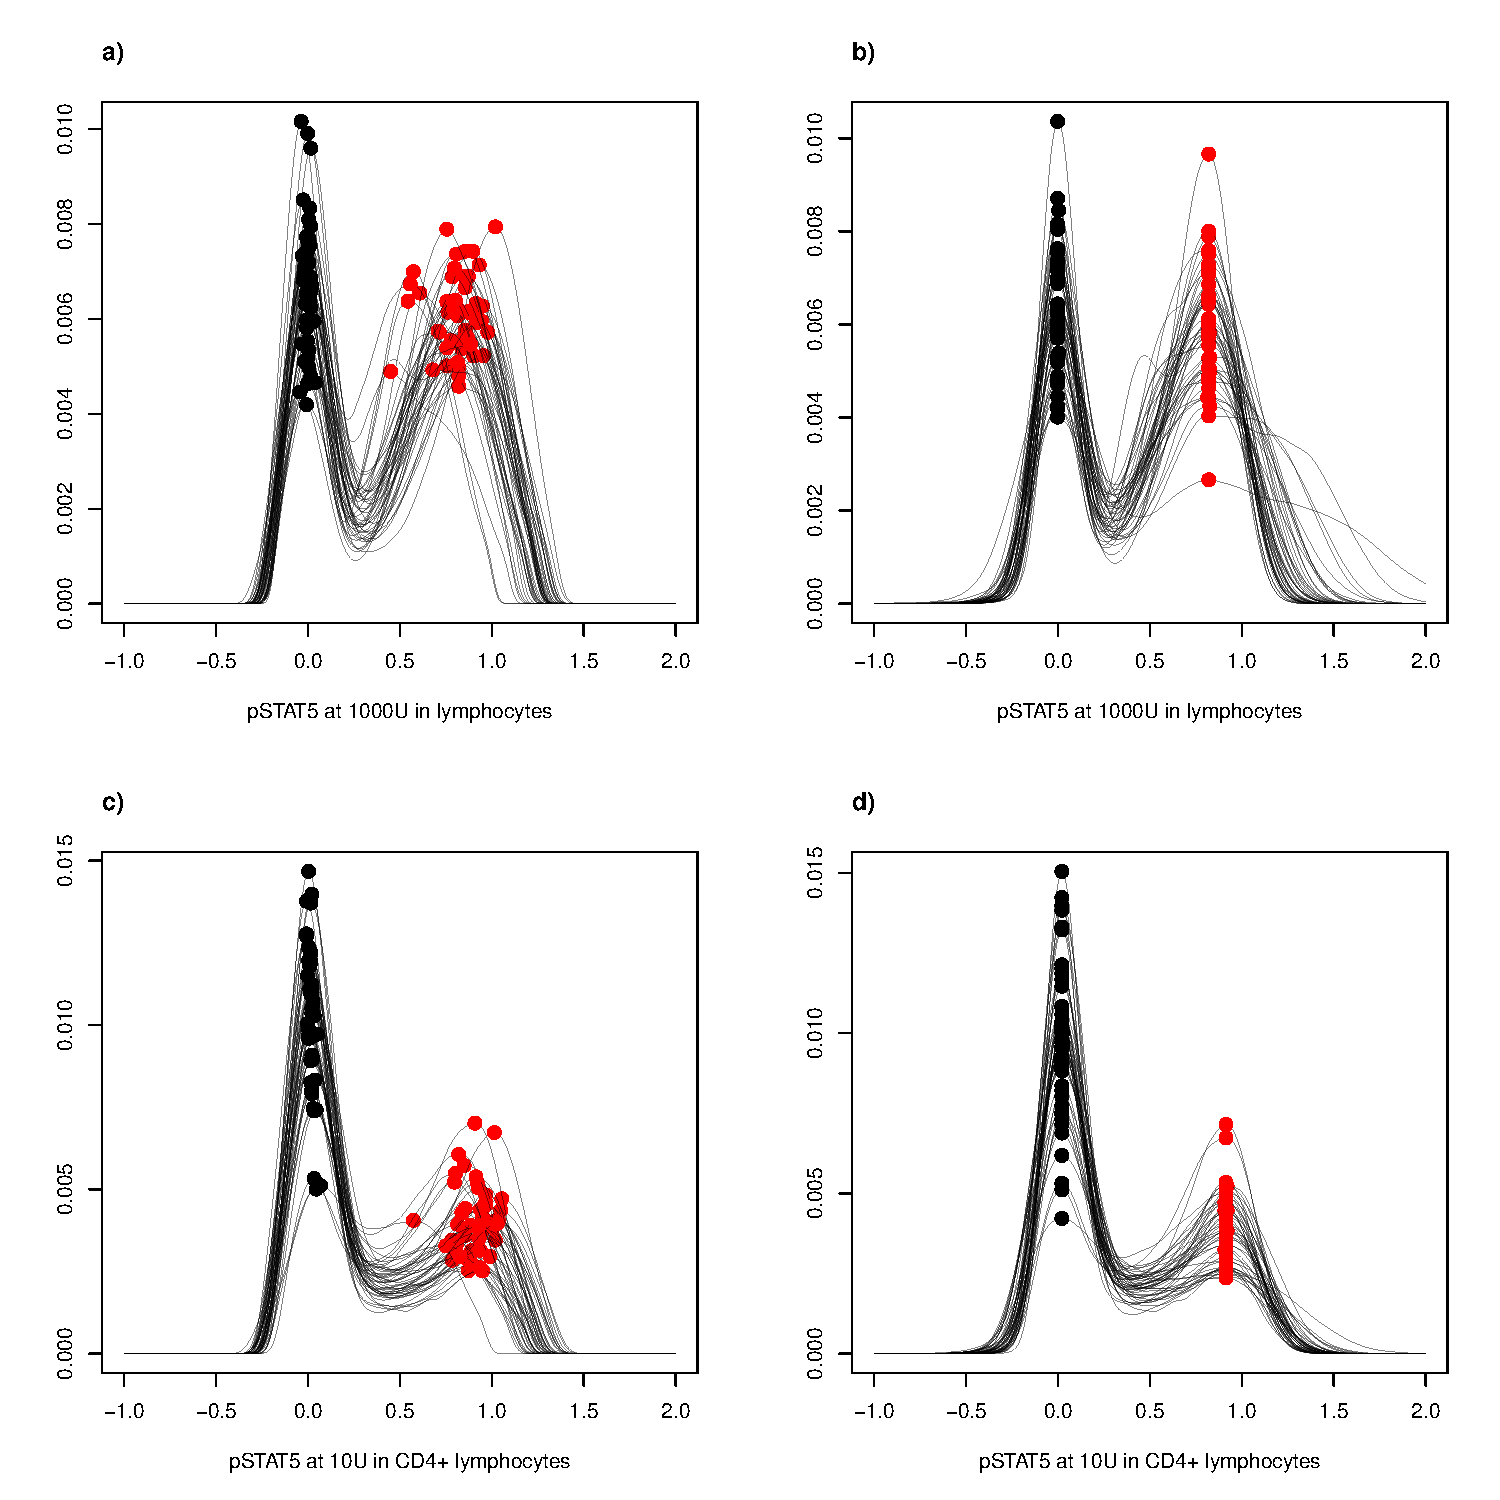
\includegraphics[scale=.5]{IL2/figures/pstat5-peak-normalisation.pdf}
    \mycaption{figure:pstat5-peak-normalisation}
    {Normalisation by peak alignment of the pSTAT5 distribution in lymphocytes (a and b) and CD4\positive lymphocytes (c and d).}
    {
      The two peaks of the pSTAT5 distribution are identified using a sliding window approach,
      in the lymphocyte sample stimulated at 1000 units (a) and in the manually gated CD4\positive lymphocyte subset stimulated at 10 units (c).
      In the normalised pSTAT5 distribution in the ungated (a) and CD4\positive lymphocyte subset (d),
      the identified peaks in (a) and (c) have been mapped to the respective medians across all peaks.
    }
\end{figure} 
In order to facilitate peak identification in the CD4\positive lymphocytes,I considered the pSTAT5 distribution at 10 units instead of 1000 units,
since the unstimulated to stimulated ratio is more even at an intermediate dose.
%since at the highest dose, most CD4\positive lymphocytes are stimulated.
%Here's an example of this method applied on simulated data where the number of peaks is known and easily identifiable (Figure~\ref{figure:simulation-peak-align}).
%The sliding window method is good for detecting local maximums while the clustering approach is better at find global splits.
%Hence we combine both approaches by using the sliding window on the partitions identified by the clustering.
%We apply mclust and pam (clara) because mclust tends to the fit the data better when the cluster are of very uneven size like example (~/pam.fail.RDAta).
Once the two peaks were identified in all samples,
%the next task is now to align for the purpose of normalisation.
%A non-linear transform could be considered so that peaks may be aligned independently, but
a linear transformation was used to exactly map the two peaks across all samples, as shown in \Cref{figure:pstat5-peak-normalisation}.
%since there are only two peaks, a linear transform is sufficient 
%After applying this transform to the previously gated pSTAT5 MFI and retested the repeatability.
%We also apply this method the pSTAT5 positivity threshold
%how?  
\clearpage


